\section*{Chapter 7}
\addcontentsline{toc}{section}{Chapter 7}

\subsection*{7.16 Consider the following set of requirements for a UNIVERSITY database that is used to keep track of students? transcripts. This is similar but not identical to the database shown in Figure 1.2.\\
\begin{enumerate}[(a)]
\item The university keeps track of each student's name, student number, Social Security number, current address and phone number, permanent address and phone number, birth date, sex, class (freshman, sophomore, ..., graduate), major department, minor department (if any), and degree program (B.A., B.S., ..., Ph.D.). Some user applications need to refer to the city, state, and ZIP Code of the student's permanent address and to the student's last name. Both Social Security number and student number have unique values for each student.
\item Each department is described by a name, department code, office number, office phone number, and college. Both name and code have unique values for each department.
\item Each course has a course name, description, course number, number of semester hours, level, and offering department. The value of the course number is unique for each course.
\item Each section has an instructor, semester, year, course, and section number. The section number distinguishes sections of the same course that are taught during the same semester/year; its values are 1, 2, 3, ..., up to the number of sections taught during each semester.
\item A grade report has a student, section, letter grade, and numeric grade (0, 1, 2, 3, or 4).
\end{enumerate}
Design an ER schema for this application, and draw an ER diagram for the schema. Specify key attributes of each entity type, and structural constraints on each relationship type. Note any unspecified requirements, and make appropriate assumptions to make the specification complete.}
\addcontentsline{toc}{subsection}{7.16}
\begin{figure}[H]
\makebox[\textwidth][c]{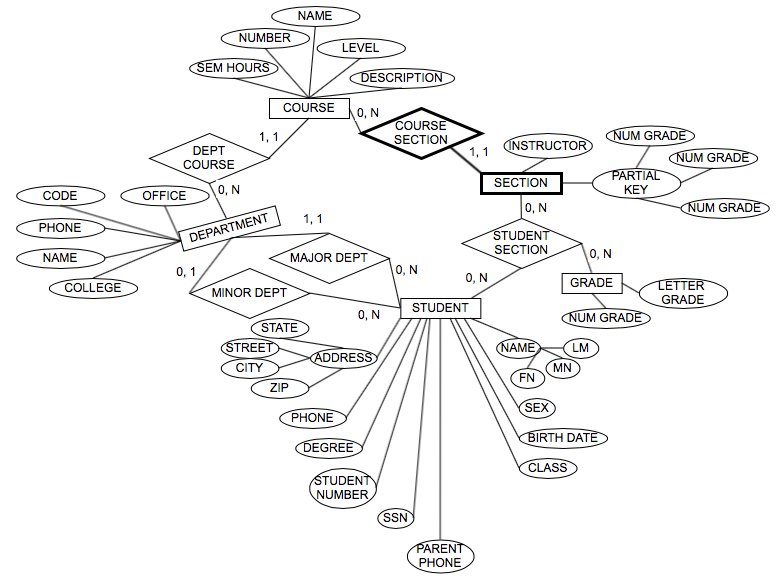
\includegraphics[width=1.2\textwidth]{images/7-16.png}}%
\end{figure}

\subsection*{7.18 Show an alternative design for the attribute described in Exercise 7.17 that uses only entity types (including weak entity types, if needed) and relationship types.}
\addcontentsline{toc}{subsection}{7.18}
\begin{center}
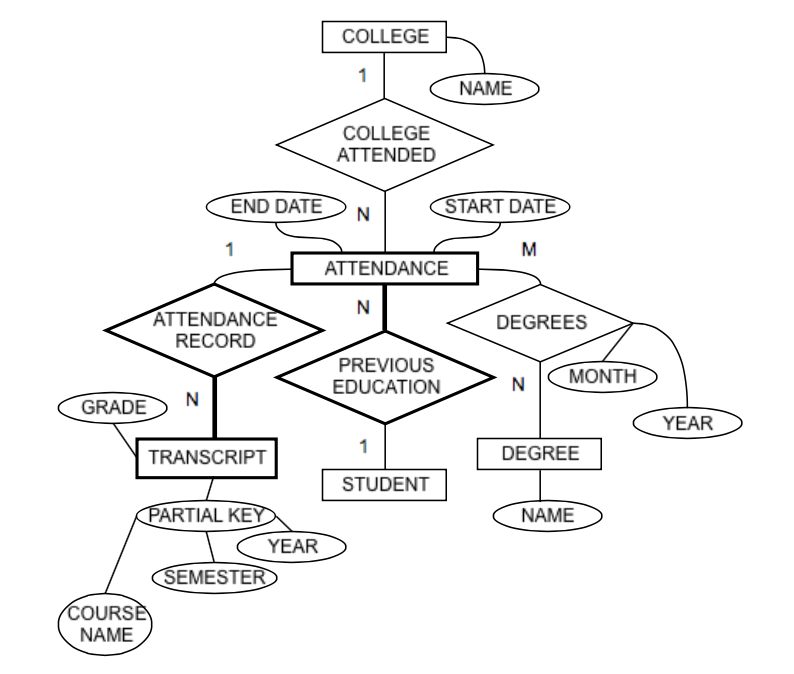
\includegraphics[width=15cm]{images/7-18.png}
\end{center}

\subsection*{7.19 Consider the ER diagram in Figure 7.20, which shows a simplified schema for an airline reservations system. Extract from the ER diagram the requirements and constraints that produced this schema. Try to be as precise as possible in your requirements and constraints specification.}
\addcontentsline{toc}{subsection}{7.19}
\begin{enumerate}
\item The given database represents any given AIRPORT. It keeps its unique Airport\_code, AIRPORT name, city and state in which it is located.
\item For each LEG\_INSTANCE, the customer RESERVATIONs includes a Customer\_name, Cphone, and Seat\_no(s).\item One can see that each FLIGHT has its unique number, its Airline, and the Weekdays on which it is scheduled.
\item Information on AIRPLANEs and AIRPLANE TYPEs are also kept. Every AIRPLANE TYPE stores the Type\_name, manufacturing Company, and Maximum Number of Seats, and AIRPORTs in which planes of that type CAN\_LAND. For each AIRPLANE, the airplane ID, Total number of seats, and TYPE are kept.
\item On a specific Date, a LEG\_INSTANCE is an instance of a FLIGHT\_LEG. After any FLIGHT\_LEG has been concluded, the DEPARTURE\_AIRPORT, ARRIVAL\_AIRPORT, the arrival times, number of available seats, and the AIRPLANE used are recorded for that FLIGHT\_LEG.
\item Any given FLIGHT has one or more FLIGHT\_LEGs. Each FLIGHT\_LEG has a DEPARTURE\_AIRPORT and ARRIVAL\_AIRPORT, with their respective Scheduled\_dep\_time and Scheduled\_arr\_time.
\end{enumerate}
